%2345678901234567890123456789012345678901234567890123456789012345678901

% chapter cha:using_legacy_tools (fold)
\chapter[Legacy astronomical packages and the VO]
{Legacy astronomical packages and the VO}
\label{cha:using_legacy_tools}
	\attributedquote{
		\dictionarydef{legacy}
					  {noun}
		{
			\begin{itemize}
				\item a thing handed down by a predecessor:
				\emph{the legacy of centuries of neglect.}
			\end{itemize}
		}
		\dictionarydef{legacy}
					  {adjective (\textsf{computing})}
		{
			\begin{itemize}
				\item Denoting software or hardware that has been
				superseded but is difficult to replace because of
				its wide use.
			\end{itemize}
		}
	}
	{The New  Oxford American Dictionary, \emph{2nd Edition}}
	
	The physical properties we can ascertain from remote
	astronomical objects are the result of careful computations on
	observed datasets, which tend to be observatory, telescope,
	instrument, and even observing mode specific. Such computations
	include background noise estimations, electron counts to
	incident flux conversions, instrument signal removal, et
	cetera.

	Many different software packages have been developed for
	performing those operations (which are commonly known as data
	reduction), and obtaining science-ready data products (i.e.,
	images which have been flux calibrated, given precise
	astrometry, et cetera), and to analyse them to get additional
	physical information. For instance, once a spectrum has been
	calibrated on the local standard of rest of the source,
	the width of an emission line can be directly correlated to
	an expansion or contraction velocity of the observed object.
	
	The development effort invested on these applications is
	enormous, and even when they have been developed using
	techniques available many years ago, and can be considered
	\emph{technologically obsolete}, the recreation of all the
	algorithms in modern languages, or on more modern GUI framework
	foundations is prohibitive, due to the extensive development
	and testing that would be needed for such a replacement.
	
	Examples of 30-year old software packages still in heavy use
	include AIPS\urlnote{http://www.aips.nrao.edu/}, a radio
	astronomical imaging package from the late seventies originally
	written in FORTRAN IV; or
	GIPSY\urlnote{http://www.astro.rug.nl/~gipsy/}, a 3D data
	analysis package for obtaining kinematic properties, whose
	development started in the early seventies, and is also written
	in FORTRAN.
	
	But the goal set for the VO is to become the entire framework
	for future astronomical and astrophysical computing, both for
	its development and its execution, becoming completely
	transparent to astronomical users.
	
	\invisiblenote{
		Talking about the Virtual Observatory will be left to
		computer scientists or astronomical software developers,
		much in the same way the Internet has become \emph{the
		internet} (without capitalising), and web applications and
		web services use it. Web applications such as Google
		Docs\urlnote{http://docs.google.com/}, Yahoo!
		Mail\urlnote{http://mail.yahoo.com/},
		YouTube\urlnote{http://youtube.com/} and the like show an
		uniform interface to the user based on HTML4/XHTML and
		JavaScript which modern web browsers can uniformly render
		and access.
	}
	
	We cannot expect, then, astronomers to embrace the VO if they
	are not able to carry over the tools they are accustomed to,
	and we cannot recreate all the existing legacy applications. We
	must, therefore, find a way to bring these legacy applications
	to operate within the VO framework. That is the scope of this
	chapter: answering \emph{How to bring legacy applications into
	the VO environment.}
	
	\invisiblenote{
		However, there are many existing astronomical applications,
		written in the pre-internet era, many of them in languages
		which do not implement network connection primitives, such
		as FORTRAN\footnote{Network programming in FORTRAN is
		performed by means of wrappers around existing C
		libraries.}, in which many man-years have been invested,
		and which the astronomical community keeps on
		using\footnote{Examples of 30-year old software packages
		still in heavy use include AIPS
		<\url{http://www.aips.nrao.edu/}>, a radio astronomical
		imaging package from the late seventies originally written
		in FORTRAN IV; or GIPSY
		<\url{http://www.astro.rug.nl/~gipsy/}>, a 3D data analysis
		package for obtaining kinematic properties, developed in
		the early seventies, also written in FORTRAN.}.
		
		 In any case, VO capabilities are very desirable, as they
		enable software packages to find, select and process data
		which the application does not need \emph{a priori}
		knowledge of where they do reside: only the metadata in the
		VO Registry is needed for service selection, and only the
		metadata provided by actual protocol queries to the service
		allow \emph{a priori} selection of the final datasets to be
		processed.
		
		 \emph{How do we provide VO capabilities to existing
		(legacy) astronomical application in the least intrusive
		way?} That is the question we wish to answer with this
		chapter.
	}
	
	\section{VO-enabling applications} % (fold)
	\label{sec:vo_enabling_applications}
		
		We must start by answering the question \emph{What is a
		VO-enabled application?} From the many VO standards and
		protocols issued by the
		IVOA\urlnote{http://ivoa.net/Documents/}, which and how
		many of them have to be implemented for us to consider an
		application is VO-enabled?
		
		We will understand that a VO-enabled application is a
		software package which:
		
		\begin{enumerate}
			\item Can read and/or write data in VOTable (and
			possibly FITS) format.
			
			\item Can query the VO Registry in order to find
			VO services or data resources, at least of one
			particular kind.
			
			\item Can call a subset of VO-registered services
			for at least one of IVOA data access
			protocols\footnote{ConeSearch, Simple Image Access,
			or Simple Spectra Access. See 
			appendix~\ref{cha:vo_protocols}.}.
		\end{enumerate}
		
		A somehow orthogonal capability is that of being able to
		communicate with other VO applications running in the same
		machine, via the \invisible{soon to be approved} Simple
		Application Messaging Protocol
		(SAMP)~\cite{2009samp.ivoav0904T}.
		
		However, an application which can use SAMP to communicate
		with others can, in fact, make use of their capabilities, and
		retrieve data which have been processed by other applications. Conversely, the
		processed results can be mixed with those of any other
		application.
		
		We can, then, consider that a VO application is just one
		which:
		
		\begin{enumerate}
			\item Can read and/or write data in VOTable (and
			possibly FITS) format.
			
			\item Can communicate with other VO applications
			through messaging, both for sending and receiving
			data from those applications.
		\end{enumerate}
		
		As we are leaving out the Registry search capability, and
		protocol calls, in order to truly VO-enable an application
		we will need to ensure that VO Registry access services, and
		ways to call VO services, are provided.
		That can be solved by either implementing or using external
		modules which can query the registry, perform data access
		queries, and return their results back to processing
		applications.
		
		Let us compare, then, the two ways we have to create
		VO-enabled applications:
		
		\begin{description}
			\item[In-application VO compatibility] In this scenario,
			we have to create a VO interface within every
			application we want to VO-enable. The following has
			to be implemented:
			
			\begin{description}
				\item[VO Registry interface] A GUI for querying the
				VO registry, looking for the kind of services the
				application can make use of. Such a GUI can be
				reused only for applications using the same
				programming language and UI framework. We must
				consider it a \emph{per application} development.
				
				\item[Changes into the User Interface] The
				application user interface (be it command-line or
				graphical) has to be changed in order to be able to
				start the new VO functions: registry query,
				image/spectra/table queries and retrieval,
				messaging with other applications, et cetera. By
				definition, this is a \emph{per application}
				development.
				
				\item[VO Data Access Layer interface] The
				application must be able to obtain data from
				existing VO services (images, spectra, or tables).
				Code to query them must be included. There are
				query interfaces written in different programming
				languages, so we will consider this a \emph{per
				language} development.
				
				\item[VOTable and FITS handling] The two approved
				data formats for the VO are the VOTable and the
				FITS file formats. Any VO application has to be
				able to handle both (many VOTables include links to
				FITS files, which hold the actual data). There are
				libraries written for many different languages for
				FITS and VOTable handling, so there is a small
				\emph{per application} development cost associated.
				
				\item[DAL to internal model interface] Data
				retrieved from the VO correspond to the DAL data
				model, while the legacy application will have an
				internal data model of its own. This is responsible
				for the VOTable/FITS data conversion into the
				actual internal representation, and it is
				completely application dependendent, and as such it
				represents a \emph{per application} cost.
				
				\item[Messaging interface \emph{(optional)}] 
				The application can also include a messaging
				interface. In that case, the DAL to the internal
				data model interface is also used by the data being
				retrieved from other applications. The messaging
				interface is based on the
				XML-RPC\urlnote{http://www.xmlrpc.com/}
				specification~\cite{1999xrpc.rept.....W}, for which
				many implementations exist in many different
				languages. The adaptation between the DAL model and
				the internal model it is the same as for the VO
				query interfaces, and includes a small amount of
				\emph{per application} adaptation in order to
				support messaging.
			\end{description}
			
			
			\item[In-application VO messaging] In this other
			scenario, we leave the interface with the registry, and
			the DAL interface to other applications, and we rely on
			messaging to get the data in and out of the
			application. In this case, the modules to be
			implemented are:
			
			\begin{description}
				\item[Minimal changes to the UI (Views) and
				Controller] Applications must be able to send data
				to compatible VO applications (applications who
				understand the kind of messages the host
				application wishes to provide), and must declare
				the kind of messages it can receive from other
				applications. The main Controller must be able to
				receive updates from the Messaging part controller.
				
				\item[Messaging interface] In this case, messaging
				is the main building block for the application:
				other applications will perform the Registry
				queries, and the calls to data access protocols.
				The results will be later messaged to the
				application.
				
				\item[VOTable and FITS handling] The messaging
				protocols use VOTables, which can include links to
				FITS files, as any other VO protocol. As mentioned
				above, there are extensive libraries for many
				different languages which can be used. We can
				consider, also, that FITS handling is a capability
				of any legacy application, so only VOTable handling
				is a true addition.
				
				\item[DAL to internal model interface] This is
				interface can be simpler than the one in the prior
				scenario, because the data origins will be the
				messaging applications. As we will see later, the
				messaging protocols impose a more strict semantics
				to the data being exchanged, allowing for a simpler
				interface.
			\end{description} 
		\end{description}
		
		%\begin{figure}[tbp]
		%	\centering
		%		\includegraphics[height=3cm]
		%		{fig/StandardMVCarchitecture.pdf}
		%	\caption{caption}
		%	\label{fig:fig_StandardMVCarchitecture}
		%\end{figure}
		
		\begin{figure}[tbp]
			\centering
			\subfloat[][]
			{
				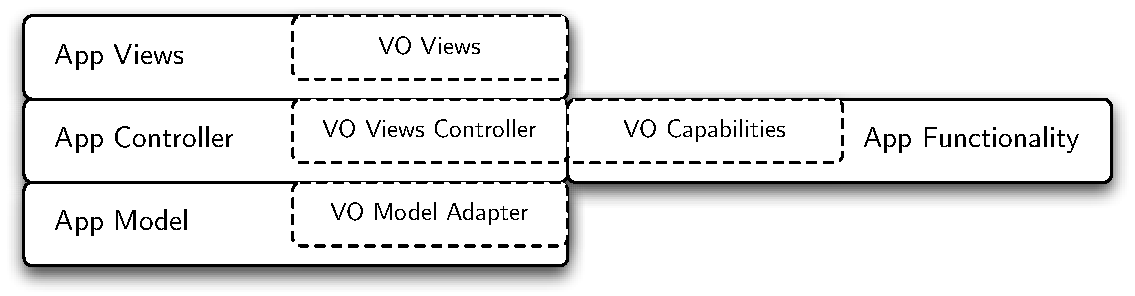
\includegraphics[width=\textwidth]
					{fig/VOappMVCarchitecture.pdf}
				%\label{fig:fig_VOappMVCarchitecture}
				\label{fig:fig_monolithic_VO}
			}
			\vfill
			\subfloat[][]
			{
				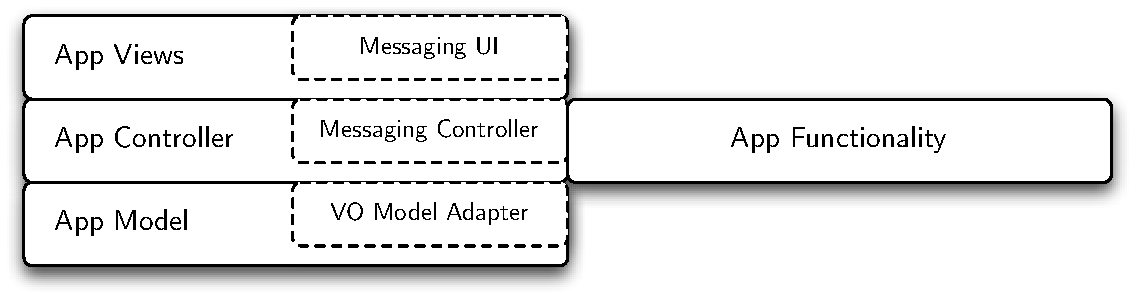
\includegraphics[width=\textwidth]
					{fig/MessagingMVCarchitecture.pdf}
				\label{fig:fig_modular_VO_capabilities}
			}
			\caption[Modules for monolithic a message-based VO-enabled
			applications]
			{
				Comparison between the functionality to be added
				and/or modified in a VO-enabled application, both
				for a monolithic approach
				\subref{fig:fig_monolithic_VO}, and for a
				messaging-based approach
				\subref{fig:fig_modular_VO_capabilities}.
			}
			\label{fig:monolithic_vs_modular_VO_capabilities}
		\end{figure}
		
		We can see these two different approaches illustrated in 
		figure~\ref{fig:monolithic_vs_modular_VO_capabilities}. 
		Figure~\ref{fig:fig_monolithic_VO} shows the monolithic
		approach to bringing legacy applications to the VO,
		with two different legacy applications and an already
		VO native application. We can see that there is a lot
		of redundancy and duplication in the development.
		
		Figure~\ref{fig:fig_modular_VO_capabilities}, on the other 
		hand, shows how a modular interface, which connects legacy
		applications via messaging protocols, decreases development
		effort, decouples the development of VO functionality, and
		provides tools which can be used with any VO messaging
		enabled application. If we assume that all legacy
		applications are able to handle FITS files, only messaging,
		VOTable handling, and DAL to internal data model
		modifications will have to be performed per application,
		while the interfaces to the VO, and all external, plug-in
		like, capabilities, can be left to external modules,
		common to all applications we might wish to update.
		
		There will be cases of applications where no modifications
		are possible, because no source code is available for them,
		or the language they are written in does not support
		web or XML-RPC interaction. In those cases, a VO downloader 
		application, ---which can act as a VO file consolidator---
		is the \emph{greatest common denominator}, and remains the
		only way to use non-VO enabled legacy applications within
		a VO workflow.
		
	% section vo_enabling_applications (end)
	
	\section{Inter-application messaging in the VO} % (fold)
	\label{sec:messaging_and_the_vo}
		
		In order to VO-enable applications through a messaging
		system,
		we wish to be able to send messages which entail particular
		actions: examples of messages and their actions would be:
		
		\begin{itemize}
			\item Issuing a \emph{data load} message, and having
			data loaded on the remote application.
			
			\item Issuing a \emph{highlight data} message, and
			have the data highlighted on the remote application.
		\end{itemize}
		
		Without taking into account the nature of the data (in 
		the VO, data is passed by means of VOTables, which might
		contain data, or link to data), it is clear that there
		might be several receivers for messages of this nature,
		so a mechanism for registering potential receivers of
		messages is needed. If the number of possible messages
		is moderate to large, an application would also need to
		declare the kind of messages it can deal with.
		
		We can see that a possible solution to this are
		publish-subscribe mechanisms, where several parties can
		act as information publishers, and several (possibly
		different) parties act as information subscribers.
		The benefits in scalability and modularity of
		publish/subscribe systems, together
		with a thorough study of their mechanisms, taxonomy, and
		predecessors, can be found in the review by
		Eugster et al.~\cite{857078}.
		
		The first messaging mechanism within the VO was an
		experiment by the VOTech project\footnote{In turn, inspired
		by the XPA (uniX Public Access,
		\url{http://hea-www.harvard.edu/RD/xpa/intro.html})
		protocol used for
		communication between tools written for the X11
		windowing system, or Tcl/Tk, or Perl packages, such as
		IRAF, or the SAOImage DS9 FITS
		viewer. IRAF, for instance, can use DS9 as its imaging
		package thanks to XPA.}, and was the PLatform for
		AStronomical Tool
		InterConnection\urlnote{http://plastic.sourceforge.net/}
		(PLASTIC)~\cite{2006pldaivoanv0606B}, a client-side
		messaging protocol.
		
		PLASTIC was based on XML-RPC messaging between client
		applications and a central hub which had to start before
		the applications could connect to it. Applications would
		register the messages they support, and would provide
		handler functions for incoming messages (callbacks).
		
		The number of defined messages was not very large, and
		by being implemented on top of XML-RPC it was easily
		ported to different languages and platforms. In fact,
		in spite of never being an IVOA standard, the number of
		applications supporting PLASTIC was very high, as the
		cost of implementing PLASTIC capabilities was very
		low.
		
		However, PLASTIC sported a number of shortcomings:
		
		\begin{description}
			\item[Hard-coded message types and parameters]
			The messages types were hard-coded in the protocol,
			making messages fixed, and not extensible. Small
			modifications to an existing message were not
			possible, as all parameters were fixed by the
			message definition.
			
			\item[Non-uniform messages] Each message had a
			number of parameters that depended entirely on
			the message type, without any governing rule.
			
			\item[Java-based typing] Data types were based on
			Java data types, instead of relying on
			platform-independent data type definitions.
			
			\item[Hard-coded transport type] PLASTIC uses
			XML-RPC as its transport protocol, making it
			impossible to use different messaging protocols
			if the need might arise (for instance, usage of
			SOAP, e-mail, or other kind of transfer protocol).
		\end{description}
		
		The answer to that was taking the best of PLASTIC, 
		which was never an IVOA standard, in spite of its 
		success, and develop a new protocol which answered
		all of the above shortcomings, while trying to be
		a drop-in replacement for PLASTIC.
		
		That protocol, an IVOA Recommendation, is the Simple
		Application Messaging Protocol
		(SAMP)~\cite{2009samp.ivoav0904T}. SAMP provides a
		messaging mechanism which is both independent of the
		actual messages being sent (which are identified by
		a unique code, the MType, and which have to be 
		standardised between applications), and independent
		on the transport mechanisms by creating different
		profiles. The Standard profile, however, uses XML-RPC
		as its transport mechanism, and resembles PLASTIC by
		using an XML-RPC based hub where applications register,
		but with enhanced message semantics.
		
		We will cover SAMP in more detail in the following
		section.
		
	% section messaging_and_the_vo (end)
	
	\section{SAMP: the Simple Application Messaging Protocol} % (fold)
	\label{sec:samp_messaging}
		
		\begin{figure}[tbp]
			\centering
				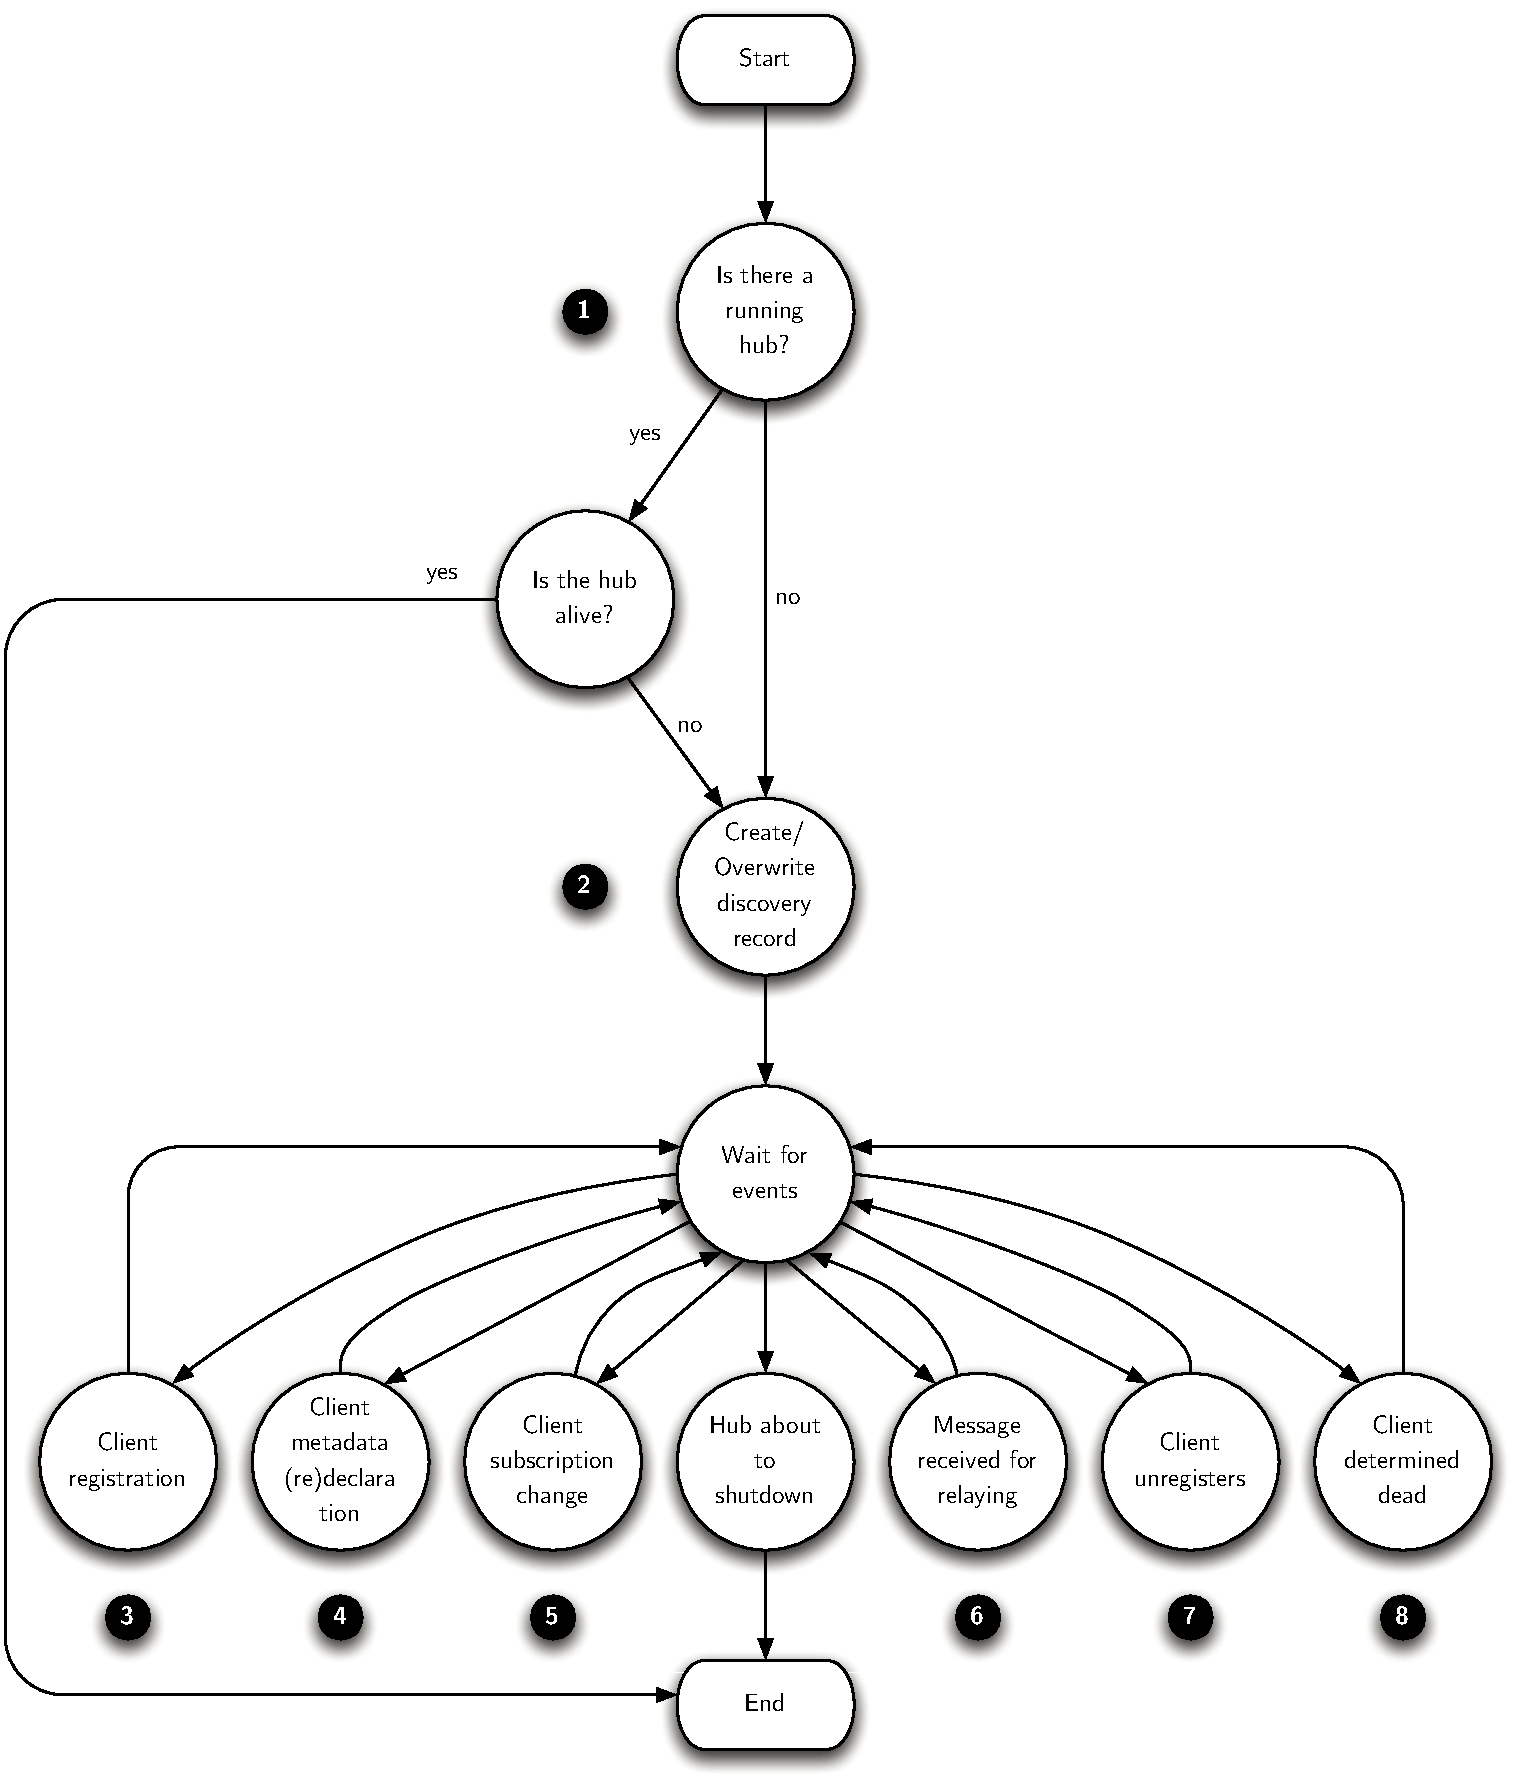
\includegraphics[width=\textwidth]
				{fig/SAMPHubLifeCycle.pdf}
				%{fig/SAMPHubLifeCycle.png}
			\caption[Life-cycle of a SAMP hub]
			{
				Life-cycle of a SAMP hub. Once determined there
				is no running, alive hub, the discovery record
				is created, and the hub waits for the different
				events it supports, until shutdown. The numbers
				on the black circles will be used to refer to
				particular steps throughout the text.
			}
			\label{fig:fig_SAMPHubLifeCycle}
		\end{figure}
		
		\begin{figure}[tbp]
			\centering
				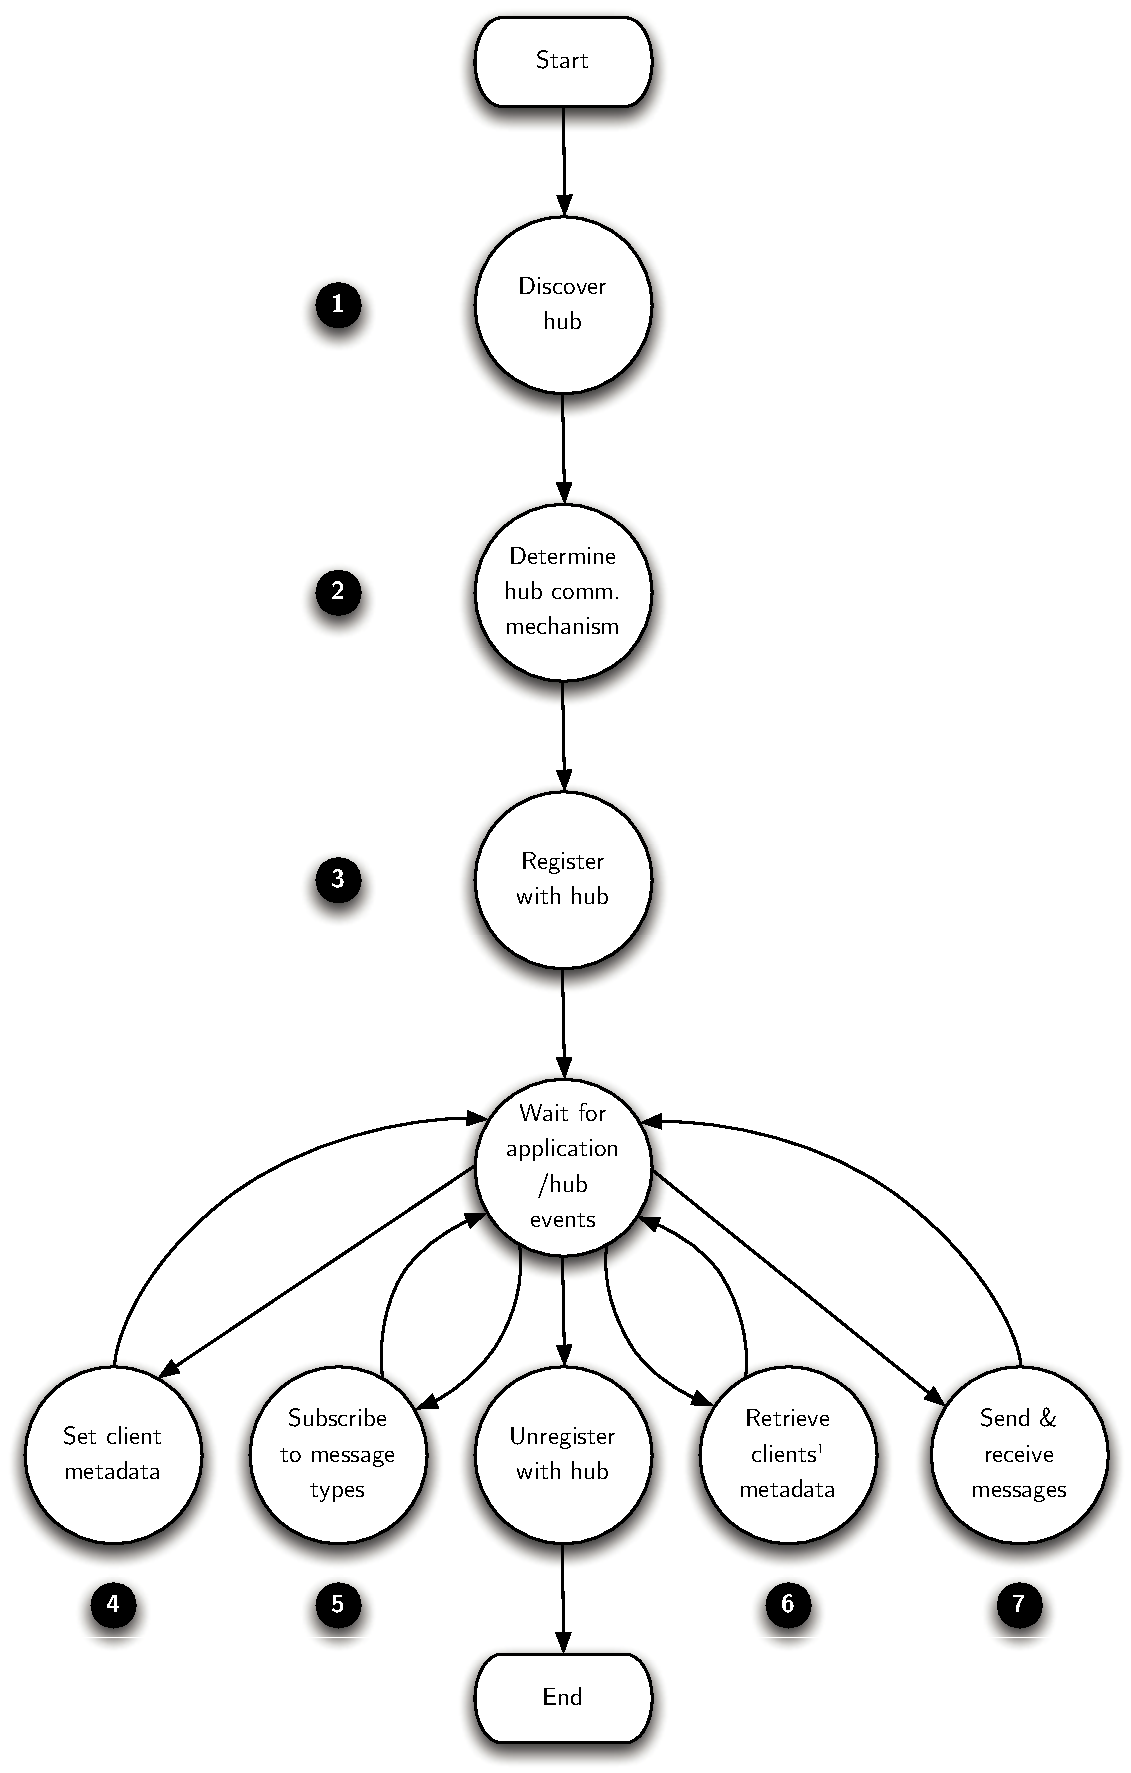
\includegraphics[width=0.75\textwidth]
				{fig/SAMPClientLifeCycle.pdf}
				%{fig/SAMPClientLifeCycle.png}
			\caption[Life-cycle of a SAMP client]
			{
				Life-cycle of a SAMP client. Once a client has
				found a hub, it registers with it, and at any
				time after registration it declares (or changes)
				metadata, subscriptions, and receives messages
				based on its subscriptions, until it unregisters
				with the hub before quitting. The numbers
				on the black circles will be used to refer to
				particular steps throughout the text.
			}
			\label{fig:fig_SAMPClientLifeCycle}
		\end{figure}
		
		
		As its predecessor, PLASTIC, SAMP is a hub-based messaging
		system, by which a intercommunication hub has to be started
		before any clients can start sending or receiving messages.
		Once the hub is started, it waits for client events, until
		shutdown condition is reached.
		
		Figure~\ref{fig:fig_SAMPHubLifeCycle} shows the complete
		life-cycle for a SAMP hub. First, the hub determines if
		there is no running, alive hub, before writing (or 
		overwriting) a new SAMP hub discovery record.
		This discovery record depends on the actual profile (or
		profiles) supported by the hub\footnote{For the standard
		profile, the hub discovery record is a file
		called \texttt{.samp}, in key=value format, stating
		the XML-RPC endpoint of the hub, among other properties.}.
		
		Once the stage has been set up, the hub waits for
		events from the clients. Supported operations are client
		registering (which gives each client a unique id for
		communication, and identification of subsequent calls),
		metadata declaration (as many times as each client
		wishes), subscription to particular message types, message
		relaying to one, several, or all clients, et cetera.
		All exchanges between SAMP applications are mediated by the
		hub, including synchronous calls between SAMP applications.
		
		Finally, when the hub is about to close, notifies all
		clients of that condition, and finally removes the
		hub discovery record, so that a new hub instance can start
		afresh.
		
		Figure~\ref{fig:fig_SAMPClientLifeCycle}, on the other hand,
		reflects the life-cycle of each SAMP client. If a hub is
		discovered\footnote{For instance, in the standard profile,
		by finding a \texttt{.samp} file at the user's home
		directory.}, it immediately enters the registration stage,
		and receives a unique identifier which allows its
		identification\footnote{Apart from that unique identifier,
		different profiles might choose additional measures in
		order to ensure there is no client spoofing. In the
		standard profile, a private key is generated by the hub
		and sent back to the client upon registration.} for
		subsequent messages. For instance, other applications might
		wish to send individual messages to applications with
		certain declared capabilities.
		
		The main difference with PLASTIC is at the message definition
		and subscription level: in SAMP, MTypes can be arbitrarily
		defined between the applications which understand them, and
		other applications can be connected to the hub without
		support for any messages other than those mandatory by the
		SAMP protocol.
		
		As the application has declared which messages does it
		subscribe to, and the function which will deal with them,
		it will only receive messages it can handle. And before
		the application is ready to quit, it should unregister
		with the hub. All application quitting events should
		handle this unregistering process, in order not to leave
		fake registered applications with the hub.
		
		Given that MTypes can be arbitrarily defined, and semantics
		and parameters are bound together by agreement between VO 
		developers within the IVOA (for public MTypes), or between
		application modules (for private MTypes), SAMP can also 
		be understood as a form of type-based publish/subscribe
		system~\cite{857078}.
		
		\invisiblenote
		{As we wish to build our system on top of the SAMP protocol,
		we need to provide a brief introduction to it.
		
		Once you have applications which are able to read and
		write both FITS files and VOTables, and which have enough
		understanding of associated metadata as to
		interoperate with VO services\footnote{That is, applications
		comply with VO data models.}, they should be able to
		consume data coming from applications in the same
		computer.
		
		An initial approach
		\begin{description}
			\item[Filesystem-based sharing] One application writes a
			file, the other application opens it. This is the
			traditional way of sharing information between
			applications. However, there is no way to bring
			attention to specific parts of the dataset, and no
			way to link actions between the two applications.
			%Some operating systems, or frameworks, such as
			%Microsoft's Object Linking and Embedding (OLE),
			%or the classic Mac OS 7 to 9 
			
			\item[Publish and Subscribe system] 
			operating systems and fram
		\end{description}}
		
		\invisiblenote{
		\todo{Speak about PLASTIC~\cite{2006pldaivoanv0606B},
		and perhaps about XPA: 
		<http://hea-www.harvard.edu/RD/PostScript/ora.ps>,
		<ftp://sao-ftp.harvard.edu/pub/rd/xpa/xpa.pdf>,
		<http://hea-www.harvard.edu/RD/xpa/>}}
		
	% section samp_messaging (end)
	
	\section{Implementing SAMP into an existing application} % (fold)
	\label{sec:implementing_samp_into_an_existing_application}
		
		We will assume the application we wish to make compatible
		with SAMP follows the Model-View-Controller (MVC) design
		pattern, because that is normally the case for GUI
		applications, and it allows for an easier discussion of
		the modifications needed.
		
		\begin{figure}[tbp]
			\centering
				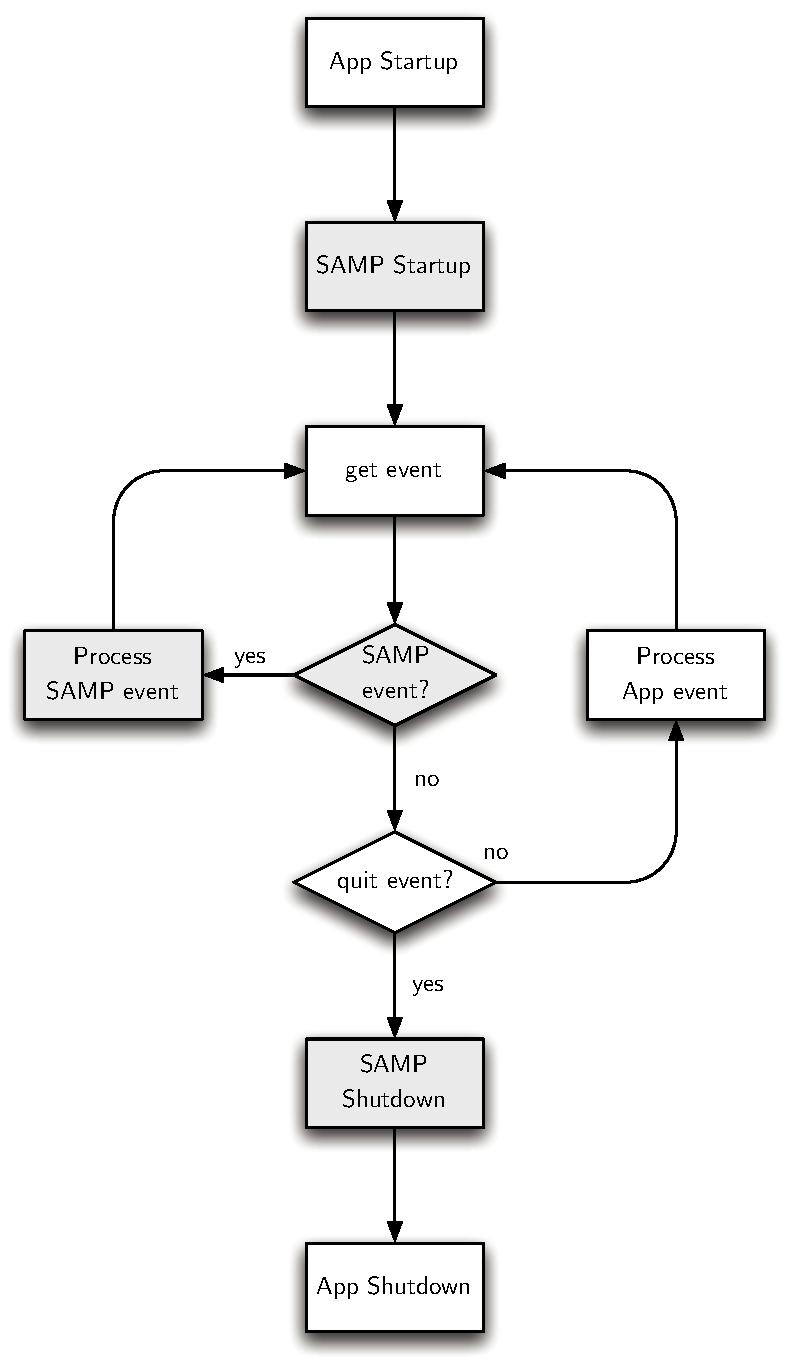
\includegraphics[height=0.6\textheight]
				{fig/SAMPEnabledAppFlow.pdf}
				%{fig/SAMPEnabledAppFlow.png}
			\caption[Simplified event flow of a SAMP-enabled
			application]
			{
				Simplified event flow of a SAMP-enabled application.
				In gray, the modules that have been introduced in
				order to provide SAMP-compatibility to an existing
				application.
				After the application has performed its start-up,
				but before entering the event-loop, we perform
				the setup of the SAMP infrastructure. We intercept
				SAMP events, in order to process them, letting the
				normal event-handling processing the rest.
			}
			\label{fig:fig_SAMPEnabledAppFlow}
		\end{figure}
		
		As the application will become a SAMP client, we need
		to add the following modules:
		
		\begin{description}
			\item[SAMP Registration module] This module would be
			added to the start-up code of the application, and
			would perform the discovery of the hub, the
			determination of the communication mechanism (in fact,
			testing that the hub corresponds to the same profile
			as the client; as we will use XML-RPC for
			communications, check the hub corresponds to the
			standard profile), and
			the registration with the hub 
			(steps 1, 2 and
			3 in figure~\ref{fig:fig_SAMPClientLifeCycle}).
			In addition, in this phase we can perform an initial
			declaration of the client metadata (step 4), and of
			the messages it subscribes to (step 5).
			
			\item[SAMP Message sending] Depending on the
			application capabilities, only a subset of possible
			MTypes will be sent. We need to create UI elements
			(buttons, pop-up menus) which provide the user with
			the possibility of sending data to other applications.
			Those pop-ups will only show applications accepting
			the messages we intend to deliver, and for that we
			will query the hub for clients' metadata (step 6).
			
			\item[SAMP Message handling] We need to implement
			the handlers for the messages we are subscribed to.
			For similitude with PLASTIC, and for extra modularity,
			a message dispatching object needs to be implemented,
			which will handle registered MTypes, which then
			dispatches the actual message to the corresponding
			handler, which in turn will make use of existing 
			application functionality to either display or
			manipulate the received message. This corresponds to
			handling of step 7.
		\end{description}
		
		In addition, some small modifications to the main view
		Controller will have to performed, so that incoming
		messages with data can be dealt with as if an \emph{open
		file} event had been issued. If the application is
		well factored, changes to the controller can be inexistent.
		
		The changes needed to the application flow are shown in 
		figure~\ref{fig:fig_SAMPEnabledAppFlow}. The main
		simplification is the \textbf{Process SAMP event} box,
		which apart from possibly reissuing application-specific
		events in order to complete event processing (i.e., for
		finishing a \emph{table load} message with an actual
		data load, in the internal data format of the application;
		if the application load messages handle FITS files, the
		changes would be minor).
		
	% section implementing_samp_into_an_existing_application (end)
	
	\section{Benefits of a SAMP-based API} % (fold)
	\label{sec:added_benefits_of_a_samp_based_environment}
		
		By implementing SAMP on an existing astronomical
		application, we have given it the opportunity to
		interact with other VO applications, and leave
		data selection in the VO to external applications.
		
		\invisiblenote
		{The main benefit from using SAMP is that we get
		modularity and messaging at the same time: there is
		less need to develop application-specific code, and
		more opportunities for code reuse.}
		
		However, given that SAMP, as a publish, subscribe, and
		messaging facility allows any kind of messages,
		by defining ad-hoc MTypes we can create new
		functionality that responds in particular ways to
		given MTypes and their parameters. This way, we can
		create a complete Application Programming Interface,
		in which instead of providing actual, byte-compiled
		functions, the functionality is provided via
		SAMP messages calls and responses.
		
		Of course, given that the standard profile for SAMP
		uses XML-RPC, we could have created such an API
		as XML-RPC instances. However, bringing the API to
		SAMP has the following advantages, both over an XML-RPC
		API or pure binary API:
		
		\begin{description}
			\item[System decoupling] By building a complete
			publish/subscribe system, we gain a three-way decoupling
			of system components~\cite{857078}:
			\begin{description}
				\item[Spatial decoupling] The \emph{spatial} term
				refers to the fact that neither publishers nor
				subscribers need to share any kind of space, or
				shared knowledge. Publishers only need to know how
				to publish, and subscribers how to subscribe to
				events.
				
				\item[Temporal decoupling] Publishers and
				subscribers do not need to orchestrate their
				interaction, and publishing is independent of
				the delivery of events to subscribers, and the
				receipt of an event to a subscribers does not need
				any interaction with the publisher.
				
				\item[Synchronism decoupling] In a true
				publish/subscribe system, such as that provided by
				SAMP, publishers are not blocked while producing
				events, and subscribers can obtain asynchronous
				notifications (via callbacks) of events: neither
				production nor consumption of messages happen in
				the main flow of control of the publishers and
				subscribers, and do not therefore happen
				synchronously.
			\end{description}
			
			\item[Modularity] The building blocks for a
			SAMP-based API are the supported MTypes, or
			families of closely related MTypes. But in any case,
			any module can provide support for one or more MTypes.
			It brings the classical \emph{do one thing well}
			motto typical from UNIX tools to the
			VO\footnote{When PLASTIC was announced, it was
			\emph{marketed} in similar terms, but many of the
			shortcomings of PLASTIC did not allow for a radical,
			modular development.}.
			
			\item[Service discoverability] In order to be
			able to receive the MType messages which conform the
			API, functional modules need to register with the
			SAMP hub. Any application can query the hub, and
			request a list of the applications (modules) which
			support particular messages. 
			\invisiblenote{The descriptions should be able to
			contain several keywords, perhaps from a UCD-like
			vocabulary, which }
			
			\item[Available for all SAMP applications] By being
			based on SAMP, a standard that many VO applications
			will implement, and thanks to the discoverability of
			SAMP-based services, we are in fact able to create a
			plug-in API for all SAMP-enabled, VO applications.
			
			\item[Easy module building] SAMP-based computing
			modules can be built in any computing language and
			operating system which provides XML-RPC support.
			In fact, as XML-RPC is an HTTP based RPC, with XML
			payloads, any language which can create sockets,
			and establish an HTTP connection, can in principle
			communicate with SAMP services\footnote{In that
			case, the most difficult part is implementing the
			callback functions.}, just by creating the XML
			as strings, and sending them over the wire in HTTP.
			This allows for SAMP module creation in the language
			the developer is more accustomed to, or having the
			best library for a particular problem.
		\end{description}
		
		The main drawback for such a message-based API when
		compared with a binary API is message latency. Function
		calls operate at the processor level (or Virtual Machine
		(VM) level, for VM-based languages such as Java, C\#, et
		cetera), while messaging needs many layers built on top of
		that.
		
		However, for interactive tasks the latency is well below
		perception limits, and is the actual computation being
		performed on the received data which will consume most of
		the time.
		
		In order to have an actual perception of the kind of
		time involved, we have used the CalcStorm testing suite
		found on the JSAMP\urlnote{\jsampurl} Java package. When
		running CalcStorm, many small clients connect to the hub,
		which understand messages for adding, subtracting,
		multiplying and dividing floating point numbers, and start
		sending calculation messages to all the rest. After
		execution, the total time elapsed is divided by the number
		of messages issued.
		
		\begin{table}[tbp]
		\begin{minipage}{\linewidth}
			\caption[JSAMP message latency tests]
			{JSAMP message latency tests. We have performed several
			timing tests with the CalcStorm testing suite of the
			JSAMP package, in a variety of situations.}
			\label{tabSAMPlatency}
		\begin{center}
		\begin{smalltabular}{cccr}
			\textbf{clients} &
			\textbf{queries} &
			\textbf{messaging kind}\footnote{\emph{sync} stands for 
											synchronous calls;
											\emph{async}
											for asynchronous;
											\emph{notify}
											for asynchronous
											notifications, without
											callbacks; and
											\emph{random} indicates
											all message kinds above
											were issued at random.}&
			\textbf{time per message} \\ \midrule
			20 & 50 & random & $10.2\pm0.3~\textrm{ms}$ \\
			\addlinespace 20 & 50 & random &
			$14.4\pm0.2~\textrm{ms}$\footnote{This result was obtained
			with an extra load on the hub caused by an additional
			testing procedure.} \\ \addlinespace 50 & 20 & notify &
			$10.7\pm0.2~\textrm{ms}$\\ \addlinespace 25 & 40 & random &
			$12.0\pm0.3~\textrm{ms}$\\ \addlinespace 1 & 1000 & random
			& $10.8\pm0.4~\textrm{ms}$\\ \addlinespace 1 & 2000 & sync
			& $10.3\pm0.3~\textrm{ms}$\\ \addlinespace 1 & 2000 & async
			& $12.6\pm0.6~\textrm{ms}$\\ \addlinespace 1 & 2000 &
			notify & $7.9\pm0.3~\textrm{ms}$\\ \addlinespace
		\end{smalltabular}
		\end{center}
		\end{minipage}
		\end{table}
		
		The results are shown on table~\ref{tabSAMPlatency},
		and where obtained on an Intel Core 2 Duo machine at
		2.4GHz, running Mac OS X 10.5.6 and a Java 1.6.0\_07 64-bit
		VM. We can see that in all cases messaging delivers
		performance which is perfectly in line with interactive
		needs: even in the slowest case, more than 68 messages per
		second could be sent and received; for computations taking
		less than messaging time to complete, real time updates can
		be provided more than 30 times per second\footnote{For
		comparison, PAL refresh rate is 25 frames per second, and
		NTSC refresh rate is 30 frames per second, which allow for
		perfectly smooth animation.}. In the best case, more than
		130 notifications per second can be delivered.
		
		We can see two additional things: First, the average cost
		for asynchronous messaging, where the calling application
		does not syncs to the response, is just 22\% higher than
		for synchronous communications. Clearly, for non-immediate
		results asynchronous messaging is the preferred, more
		robust solution, but for fast enough calculations
		synchronous messaging works better.
		
		Second, as the notify test just provides a message,
		without waiting for computation results, it can be shown
		that messaging overhead for this very simple computations
		is around 77\%. This includes the creation of the message,
		parsing of the arguments, and return of the message in XML
		format. For heavier computations, the corresponding
		messaging overhead would strongly decrease.
		
		\invisiblenote{
		 we
		obtained a figure of \invisiblenote{10687,9968,10041µs}
		$10.2\pm0.3~\textrm{ms}/\textrm{message}$ under a
		medium-load status (generated by the CalcStorm test
		itself\footnote{CalcStorm, by default, generates 20
		Calculator services which perform 100 calls between each of
		them, choosing at random between synchronous and
		asynchronous messages, and pure notifications.}), and
		\invisiblenote{14220,14517,14540µs}
		$14.40\pm0.16~\textrm{ms}/\textrm{message}$ under a
		medium-to-high-load status\footnote{Simulated by
		running simultaneously a JSAMP HubTester instance,
		another JSAMP hub testing tool.}.}
		
		We have to take into account that CalcStorm timing takes
		into account the time needed to create the clients,
		register them with the hub, perform all queries, and
		unregister them. Even when that is taken into account, all
		of that can be performed in $176\pm9~\textrm{ms}$. Most of
		the time, there are additional, higher latencies, involved
		in the kind of interactivity supported by SAMP.
		
		One more thing to note: messaging is eminently parallel, a
		very desirable feature in the days of multi-core: going
		from one core to two cores\footnote{With a monitoring
		application on to see load on each CPU}, latency jumped
		from $7.56\pm0.14~\textrm{ms}$ to $13.7\pm0.4~\textrm{ms}$,
		resulting in 1.8~times slowdown, well in line with the core
		decrease. As each execution unit can reside in different
		cores, and message parameters have to be copied in order to
		create the actual XML message, and then parsed again by the
		receiving end, there are far less opportunities for
		exploiting core-locality, providing many more opportunities
		for gains by parallelisation.
		
	% section added_benefits_of_a_samp_based_environment (end)
	
	\section{Conclusions} % (fold)
	\label{sec:legacy_conclusions}
		
		In this chapter, we have shown that, in order to bring
		astronomical legacy application into the VO one of the
		less intrusive techniques is building VO-compatible
		messaging in them, and let other applications and modules
		perform the actual interfacing with the VO.
		
		That results in a faster adaptation of legacy applications
		to the VO environment, and in a much more modular, and
		more parallel, development of VO functionality.
		
		However, in order to actually bring applications into the
		VO we need the following items to exist:
		
		\begin{description}
			\item[VO Downloader] Or file consolidator. As mentioned
			ealier, all legacy astronomical packages are able to
			read and/or write FITS files. Being able to retrieve
			both FITS files, and VOTables for later conversion, are
			the bare minimum for compatibility with the VO.
			
			\item[VO Registry and DAL module] For applications which
			have been enhanced with SAMP messaging, but have not
			implemented queries to the VO, a GUI providing access
			to data services in the VO is the way to access to
			VO data. In this module data sources will be selected,
			and once queried on a single or multiple cones, the
			data provided will be sent by SAMP messaging to
			accepting parties.
			
			\item[VOTable to FITS converter] Similar to the
			VODownloader, a VOTable to FITS converter is needed
			for providing VO compatibility with applications which
			cannot be modified.
			
			\item[Additional API] The modules above conform the bare
			minimum to provide VO compatibility for GUI, SAMP based
			applications. However, as we can provide units which
			perform arbitrary computations on the parameters
			provided (asynchronous messaging supports long execution
			times, and the called module could issue a different
			message to the calling application, depending on the
			semantics of the message sent), we can built arbitrary
			modules.
			
			In this thesis, we will demonstrate support for the
			following modules:
			
			\begin{description}
				\item[Name to coordinates resolver] Sesame is a
				web-service hosted by the CDS which provides
				coordinates for galactic and extragalactic objects,
				based on the name of the object. We will provide a
				module which will understand a series of object
				solving messages, and will deliver different kinds
				of answers.
				
				\item[FFT module] An FFT module will be developed,
				which uses both custom MTypes, but also
				\method{table.load.*} and \method{image.load.fits}
				messages, and sends back the result as
				corresponding table or image load messages to the
				calling application, so that arbitrary SAMP
				applications can make use of this computation
				facility.
			\end{description}
			
			We will provide a Python wrapper to call these
			modules from Python source code, and some of the
			modules will be written in Python as well. However,
			as the API is based on SAMP messages, any language can
			be used to write the modules, and the modules can be
			run simultaneously or one by one, as only the modules
			supporting the messages and computations we are 
			interested in need to be  \invisible{running and}
			registered with the hub.
		\end{description}
		
		In the following chapter, we will define the actual API,
		and the implementation, for the modules established above.
		
	% section legacy_conclusions (end)
	
	%As we have reiterated throughout this thesis, astrophysics is the
	%science of carefully treating received light in order to infer
	%physical properties from observed objects.
	%
	%We learn the
	%information embedded in that light by measuring the effects of
	%light on detectors, and careful processing of the light, then,
	%means we must take into account the effects of absence of
	%light on detectors, and the effects of exposing detectors with 
	%a uniform light source. Then a calibration of electron counts or 
	%voltage levels, depending on the kind of detectors, has to be 
	%performed in order to correlate that signal with the actual
	%photon flux in the received band.
	%
	%All mentioned tasks are typically performed by astronomical data
	%reduction packages, and those are just for getting a
	%correspondence between sensor output and emitted flux. After
	%that, high level analysis packages can derive 2D or 3D
	%kinematics from the data being provided.
	%
	%As a result, there is a very large number of astrophysical
	%software packages which have been developed throughout
	%the years, both for use for data from a few telescopes, or
	%for data coming from a whole family of instruments, with
	%different algorithms for data processing which might be
	%simple in some cases, or quite sophisticated in another, but
	%rely on astronomical and physical assumptions which
	%have to be kept during the processing\footnote{This is
	%particularly true for packages which rely on models of the
	%physical process, using inversion mechanisms for fitting a
	%multidimensional function from the space of parameters we wish
	%to obtain into the space of measurable properties.}.
	%
	%Once a package and/or algorithm has been debugged and
	%established, it can
	%keep being used for decades\footnote{Examples abound: AIPS 
	%<\url{http://www.aips.nrao.edu/}>
	%is a
	%radio astronomical imaging package from the late seventies 
	%originally written in FORTRAN IV,
	%while IRAF <\url{http://iraf.noao.edu/}> is an optical data 
	%reduction package from the middle
	%eighties, and GIPSY <\url{http://www.astro.rug.nl/~gipsy/}>
	%is a 3D data kinematics analysis package
	%from the early seventies, also written in FORTRAN.}.
	%That allows for easy comparison
	%of results from different teams using the same implementation,
	%and creates a barrier for changing underlying technologies.
	%
	%Indeed, 
	%re-implementing an algorithm in a new language or technology
	%is error-prone. And legacy applications in astronomy keep not
	%only their algorithms intact, but their user interfaces. This
	%makes it difficult for an emerging standard such as the
	%Virtual Observatory to be implemented 
	%
	%many man-years have been invested in
	%updating the astronomical knowledge embedded in their operation.
	%Trying to recreate such tools in more modern languages
	%(languages capable of operating with the Internet, for example)
	%would result in the introduction of calculation bugs, and the
	%investment of a lot of testing time in the ported applications.
	
%	\section{Development considerations} % (fold)
%	\label{sec:development_considerations}
%	
%		Not all legacy applications are equal from the point of
%		view of the ease of their porting to the VO.
%
%		A first classification can be made on the availability of
%		source code for the application (or a contact with the
%		application maintainer), and latter on the capabilities of
%		the programming language the application has been written
%		in:
%	
%		\begin{enumerate}
%			\item Applications without available source code nor
%			maintainer.
%		
%			\begin{enumerate}
%				\item Applications with an RPC interface or public
%				API.
%				
%				 \item Applications without an RPC or public API.
%			\end{enumerate}
%	
%			\item Applications with available source code (or
%			maintainer)
%	
%			\begin{enumerate}
%				\item Applications written in Internet and XML-aware
%				languages.
%				
%				 \item Applications written in non-Internet or
%				XML-aware languages.
%			\end{enumerate}
%		\end{enumerate}
%	
%		This classification affects the different courses of action
%		we can take for making the legacy application VO-compatible:
%	
%		\begin{enumerate}
%			\item Application source code is not available, and no
%			contact is possible with the original application
%			developer:
%	
%			\begin{enumerate}
%				\item If the application does not have an RPC
%				interface, nor a public API, the only possible
%				course of action is having an external VO data
%				downloader, and rely on the compatibility with
%				either FITS files, or with tabular data formats such
%				as CSV, TST, et cetera. Interoperation with other VO
%				tools is only possible by importing products in the
%				most suitable tool. This is the case for many
%				applications.
%				
%				 \item If the application provides a public RPC
%				interface, or API, building a module that translates
%				external petitions into the application is feasible,
%				depending on the published interfaces. All of the
%				data transformation into the application specific
%				data models and data formats must be performed
%				outside of the application.
%				
%				 In this case we have two sub-cases:
%				
%				\begin{enumerate}
%					\item The RPC interfaces/API allow for callback
%					methods. This is the best case for applications
%					for which it is not possible to get access to
%					the source code. An intermediate VO module can
%					send data to the legacy application, but can
%					also register callback methods to be called when
%					the legacy application wants to send data back.
%					
%					\item RPC interfaces/API do not allow for
%					callback methods. In this case, the intermediate
%					VO module can send data to the legacy
%					application, but the application cannot interact
%					with the VO.
%				\end{enumerate}
%				
%			\end{enumerate}
%	
%			\item Application source code is available (or the
%			maintainer wishes to bring his tool into the Virtual
%			Observatory).
%			
%			The corresponding two sub-cases depend on the programming
%			language capabilities:
%			
%			\begin{enumerate}
%				\item If the programming language has libraries to
%				interact with the Internet, and to manipulate XML
%				and FITS files, we are in the best possible case, as
%				the application will not only be able to receive
%				data from the VO (via an established public API, or
%				by creating one), but also to send queries to the VO
%				and retrieve data (creating the appropriate query
%				methods). We will use this approach for applications
%				based on Java or modern, internet-aware scripting
%				languages such as Python.
%				
%				 \item If the programming language lacks libraries
%				to interact with the Internet, or for manipulating
%				XML and FITS files, those will have to be built
%				first, or rely on a VO downloader as in the \emph{no
%				source code} case.
%			\end{enumerate}
%	
%		\end{enumerate}
%		
%	
% section development_considerations (end)
	
%	\section{Decisions} % (fold)
%	\label{sec:decisions}
%		
%		In this thesis, we have created a modular VO tool which
%		decouples VO interaction from the adaptation of the VO
%		data model to the internal application data model.
%	
%		With this approach, three modules are needed:
%	
%		\begin{itemize}
%
%			\item a VO interaction module is created, with an
%			emphasis on radio astronomical data and in both GUI and
%			scripting operation, which can be used either
%			standalone or for providing legacy (or new) applications
%			with VO services;
%		
%			 \item an application-specific module, either built
%			inside the application source code, or calling the
%			application API or callbacks, which communicates with
%			the VO interaction module for VO services.
%		
%			 \item and several helper modules: a generic VO Downloader
%			which can be used for applications for which the only VO
%			compatibility is the FITS file; a VO Data Access and Query
%			module; which is used to retrieve the data for all other
%			modules; and a sample calculation module, which can
%			provide advanced calculation services to VO applications,
%			but also to any application able to call XML-RPC services.
%
%		\end{itemize}
%		
%		We will describe those modules in the next chapter, 
%		together with the VO Downloader, and we will
%		describe how to create the application-specific module for
%		a particular application, the \massa{} spectral analysis tool,
%		in chapter~\ref{cha:massa_and_movoir}.
	
	
	
	% In any case, the best possible outcome for bringing a legacy
	% application into the VO is being able to implement one of
	% IVOA's messaging protocols, either PLASTIC or SAMP, and
	% integrating the messaging mechanism in the controller of the

	% In the following sections, we will show two examples of
	% bringing legacy applications into the VO, one corresponding
	% to the closed-source kind, and another one corresponding to
	% an application written in Java (a programming language with
	% libraries for XML, FITS, and Internet interaction.)
	% 
	%  But first, we will analyse exactly what needs to be
	% provided for both kinds of applications, so that a common
	% strategy can be built.
	
	% section decisions (end)
	
%	\section{Common features of a VO wrapper module} % (fold)
%	\label{sec:common_features_of_a_vo_wrapper_module}
%	
%	% section common_features_of_a_vo_wrapper_module (end)
	
%	\section{An example: \massa{}} % (fold)
%	\label{sec:an_example_massa}
%	
%	\subsection{What is \massa{}?} % (fold)
%	\label{sub:what_is_massa}
%	
%	% subsection what_is_massa_ (end)
%	
%	\subsection{Internal \massa{} data model} % (fold)
%	\label{sub:internal_massa_data_model}
%	
%	% subsection internal_massa_data_model (end)
%	
%	\subsection{Coupling \massa{} with PLASTIC/SAMP} % (fold)
%	\label{sub:coupling_massa_with_plastic_samp}
%	
%	% subsection coupling_massa_with_plastic_samp (end)
%	
%	
%	% section an_example_massa (end)
%	
%	\section{Another example: \textsc{GIPSY}} % (fold)
%	\label{sec:another_example_gipsy}
%	
%		The \emph{Groningen Image Processing
%		SYstem}~\cite{1980tdp..conf..169S, 1985daa..conf..271A,
%		1992ASPC...25..131V, Terlouw:1992lq} (GIPSY) is a software
%		package developed in the seventies at the Kapteyn Institute
%		of Groningen for scientifically treating the data cubes of
%		the Westerbork Synthesis Radio Telescope (WRST) in order to
%		extract physical parameters (rotation curves, warped or
%		non-warped disc models, velocity fields...) by fitting
%		spectral lines to emission intensity, calculating relative
%		speeds in observed galaxy reference frame, and then fitting
%		a disc and a bulge distribution.
%		
%		 The core GIPSY system was originally written in C, while
%		many processing routines where written in FORTRAN, as many
%		scientific processing applications of the time. GIPSY
%		contains many algorithms which are really useful for the
%		scientific exploitation of radio astronomical data cubes,
%		such as:
%		
%		 All of these tools share a common data model ---see section
%		on the GIPSY data structure (GDS)
%		in~\cite{1992ASPC...25..131V}--- for the data cubes they can
%		work with, which allows slicing the cube in one or more
%		dimensions, and with variable sizes, so that slices
%		consisting of single planes, single rows, or even single
%		pixels, in any dimension, can be tagged with custom
%		metadata. All of this different slices are kept together in
%		the same file, and the different subsets and tags are kept
%		separate of the data.
%		
%		 GIPSY has a scripting language, COLA (\emph{COntrol
%		LAnguage}), that allows both interactive and non-interactive
%		scripts to have access to the GDS, and either call existing
%		GIPSY tasks with parameters fixed in the script, retrieving
%		results, or perform calculations on their own.
%		
%		 In recent times, GIPSY has been enhanced with Python
%		bindings for COLA, something that allows using GIPSY
%		routines, and GDS access, within the Python environment, and
%		to import Python packages from the COLA environment. As we
%		can see from our discussion on the properties of legacy
%		packages, this opens the door of the VO for GIPSY, as Python
%		is an Internet and Web services aware language, for which
%		many VO tools exist.
%		
%		 \todo{Check assertion before.}
%			
%			 The planned strategy for updating GIPSY and incorporating
%            VO capabilities is the following:
%	
%		\begin{enumerate}
%			\item Complete GIPSY Python bindings, so that both
%			Python scripts can use GIPSY facilities, and COLA
%			scripts can make use of Python modules.
%			
%			 \item Rewrite most existing COLA scripts as Python
%			modules. Modules rewritten in Python will automatically
%			earn 64-bit cleanness, and
%			
%			 \item Create Python scripts to perform the following VO
%			functions:
%			
%			\begin{itemize}
%				\item Perform ConeSearch queries on the region of
%				the sky being viewed, or any other the script might
%				ask for.
%				
%				 \item Send PLASTIC and/or SAMP messages to other
%				applications with the content of image planes or
%				spectra.
%				
%				 \item Enhance GIPSY controller to be PLASTIC and/or
%				SAMP aware, so that it can receive data coming from
%				other VO applications.
%			\end{itemize}
%		\end{enumerate}
%	
%		As there is no IVOA recommended data model for cubes, we
%		will try to standardise a data format that is compatible
%		with ALMA and existing tools. There is some work already
%		performed for standardising IFUs 3D spectra, such as the
%		Euro3D data format \cite{2004AN....325..159K}.
%		
%		 This author has entered the IVOA Data Modelling Working
%		Group with the aim of contributing both with the RADAMS, and
%		with a future 3D metadadata standard for 3D datasets within
%		the VO.
%	
%	
%	% section another_example_gipsy (end)
%	
%	\section{Conclusions} % (fold)
%	\label{sec:legacy_conclusions}
%	
%	 - For legacy apps, th
%	
%	% section legacy_conclusions (end)

% chapter using_legacy_tools (end)
